\documentclass[journal]{IEEEtran}

\usepackage{csquotes}

% *** CITATION PACKAGES ***
%
\usepackage{cite}
% cite.sty was written by Donald Arseneau
% V1.6 and later of IEEEtran pre-defines the format of the cite.sty package
% \cite{} output to follow that of IEEE. Loading the cite package will
% result in citation numbers being automatically sorted and properly
% "compressed/ranged". e.g., [1], [9], [2], [7], [5], [6] without using
% cite.sty will become [1], [2], [5]--[7], [9] using cite.sty. cite.sty's
% \cite will automatically add leading space, if needed. Use cite.sty's
% noadjust option (cite.sty V3.8 and later) if you want to turn this off
% such as if a citation ever needs to be enclosed in parenthesis.
% cite.sty is already installed on most LaTeX systems. Be sure and use
% version 4.0 (2003-05-27) and later if using hyperref.sty. cite.sty does
% not currently provide for hyperlinked citations.
% The latest version can be obtained at:
% http://www.ctan.org/tex-archive/macros/latex/contrib/cite/
% The documentation is contained in the cite.sty file itself.





% *** GRAPHICS RELATED PACKAGES ***
%
\ifCLASSINFOpdf
  \usepackage[pdftex]{graphicx}
  % declare the path(s) where your graphic files are
  \graphicspath{{./pdf/}{./jpeg/}}
  % and their extensions so you won't have to specify these with
  % every instance of \includegraphics
  \DeclareGraphicsExtensions{.pdf,.jpeg,.png}
\else
  % or other class option (dvipsone, dvipdf, if not using dvips). graphicx
  % will default to the driver specified in the system graphics.cfg if no
  % driver is specified.
  \usepackage[dvips]{graphicx}
  % declare the path(s) where your graphic files are
  \graphicspath{{./eps/}}
  % and their extensions so you won't have to specify these with
  % every instance of \includegraphics
  \DeclareGraphicsExtensions{.eps}
\fi
% graphicx was written by David Carlisle and Sebastian Rahtz. It is
% required if you want graphics, photos, etc. graphicx.sty is already
% installed on most LaTeX systems. The latest version and documentation
% can be obtained at: 
% http://www.ctan.org/tex-archive/macros/latex/required/graphics/
% Another good source of documentation is "Using Imported Graphics in
% LaTeX2e" by Keith Reckdahl which can be found at:
% http://www.ctan.org/tex-archive/info/epslatex/
%
% latex, and pdflatex in dvi mode, support graphics in encapsulated
% postscript (.eps) format. pdflatex in pdf mode supports graphics
% in .pdf, .jpeg, .png and .mps (metapost) formats. Users should ensure
% that all non-photo figures use a vector format (.eps, .pdf, .mps) and
% not a bitmapped formats (.jpeg, .png). IEEE frowns on bitmapped formats
% which can result in "jaggedy"/blurry rendering of lines and letters as
% well as large increases in file sizes.
%
% You can find documentation about the pdfTeX application at:
% http://www.tug.org/applications/pdftex


% *** ALIGNMENT PACKAGES ***
%
\usepackage{array}
% Frank Mittelbach's and David Carlisle's array.sty patches and improves
% the standard LaTeX2e array and tabular environments to provide better
% appearance and additional user controls. As the default LaTeX2e table
% generation code is lacking to the point of almost being broken with
% respect to the quality of the end results, all users are strongly
% advised to use an enhanced (at the very least that provided by array.sty)
% set of table tools. array.sty is already installed on most systems. The
% latest version and documentation can be obtained at:
% http://www.ctan.org/tex-archive/macros/latex/required/tools/


% *** PDF, URL AND HYPERLINK PACKAGES ***
%
\usepackage{url}
% url.sty was written by Donald Arseneau. It provides better support for
% handling and breaking URLs. url.sty is already installed on most LaTeX
% systems. The latest version and documentation can be obtained at:
% http://www.ctan.org/tex-archive/macros/latex/contrib/url/
% Basically, \url{my_url_here}.


% correct bad hyphenation here
\hyphenation{op-tical net-works semi-conduc-tor}

\begin{document}

\title{An overview of the ongoing IPv6 deployment}

\author{Raphael~Javaux, University of Liege}

% The paper headers
\markboth{Network Measurement and Monitoring, March~2014}
         {An overview of the ongoing IPv6 deployment}
% The only time the second header will appear is for the odd numbered pages
% after the title page when using the twoside option.

\maketitle

\begin{abstract}
    We resumed in this paper four sources of IPv6 maturity measurements spanning
    from 2005 to 2012 and we completed them with some more recent results. \\
    We concluded that the IPv6 network adoption is now evolving in an
    enthusiastic albeit slow way and that any observable IPv6 speed deficiency
    is not caused by the protocol but by the current immaturity of the network
    topology.
\end{abstract}

% \begin{IEEEkeywords}
% IEEEtran, journal, \LaTeX, paper, template.
% \end{IEEEkeywords}

\section{Introduction}

\IEEEPARstart{A}{}s of today, the three major regional Internet registries
(APNIC, ARIN \& RIPE) exhausted their respective allocated IPv4 address spaces.
This major event is making the new (yet two decades old) IPv6 protocol adoption
unavoidable. \\
As January 2014, according to Google statistics\cite{google:ipv6}, only 3\%
of their users were accessing their services using IPv6. As low as this number
is, it is increasing exponentially, getting a twenty fold improvement since
January 2009, which proves that the IPv6 revolution is clearly ongoing. \\
This paper is intended to give an overview of the current state of the IPv6
deployment all along with a summary of the improvements which have been done
for the past ten years. Its primarily based on four sources,
\cite{paper1}, \cite{paper2}, \cite{paper3} and \cite{paper4}, spanning from
mid-2005 to the end of 2012. \\

Section \ref{primordial} goes through a report of the early stages of the IPv6
adoption. \\
Section \ref{penetration} talks about the penetration of the IPv6 protocol
in end-users (clients) and in the network (ASes and routers). \\
Section \ref{performances} compares the performances of IPv6 to IPv4.

\section{The primordial IPv6 network}
\label{primordial}

\subsection{A small network}

During the early stages of IPv6, the network was highly sparse and only a few
peering points were available to transmit intercontinental packets. \\
Engineers made a study on the reachability and performance of dual-stack web
servers when contacted from the Chinese Education and Research Network in
2005\cite{paper1}. They noticed that the link to some European countries was
very poor when compared in term of packet loss to its IPv4 counterpart
(see Fig. \ref{fig:packet_loss}). The reason was that most IPv6 packets going
to Germany (DE), Ireland (IE) or France (FR) were using a restricted set of
common links/tunnels (see \ref{tunnels}) with a very high packet loss rate. \\
That is, only a few transit operators and content providers were providing IPv6
connectivity and a lot of traffic was done using tunnels.

\subsection{Early adopters}
\label{early}

Using machine learning techniques, \cite{paper4} were able to organize ASes by
their owner's type of business. They analyzed IPv6 and IPv4 ASes history
and classified ASes in four groups: large transit providers (LTP), regional
transit providers (STP), content providers (CAHP) and edge customers (EC). \\
The classification over time is shown in Fig. \ref{fig:as_types}. We can see
that the IPv4 network has always been widely dominated by edge customers while
the IPv6 network has been ruled by transit and content providers till around
2010. This implies that the adoption of IPv6 mainly happened in the core network
in the early stages, with some lags on the edges. Edge customers are now
catching up as they started following an exponential growth since 2010 and the
monthly number of new IPv6 ASes is now beyond the IPv4 one. More details about
the network penetration is given in \ref{network_penetration}. \\
Another historical tendency was the early adoption of IPv6 by European and Asian
operators when compared to others. This was probably due to a favorable
regulatory environment in these regions. Either in IPv6 or IPv4, RIPE is the
leading RIR in number of ASes. \\
At the time of this writing, 17.5\% of global ASes are announcing an IPv6
prefix. ARIN is still strongly lagging behind APNIC and RIPE by only announcing
13.5\% of its prefixes whereas the two others are announcing 20.5\% and 20\% of
their prefixes, respectively\cite{ripe:ipv6stats}.

\subsection{The initial dominance of IPv6 over IPv4 tunnels}
\label{tunnels}

From the beginning of its deployment up until a few years ago, IPv6 was heavily
relaying on tunnel mechanisms (mostly \textit{6to4} and \textit{Teredo}) to
carry packets between two hosts. \\
This presence of tunnels was, along with the sparsity of the initial mesh, the
main explained cause for a smaller average numbers of hops observed between two
hosts in IPv6 (8.7 hops versus 17.5 for IPv4) in old \cite{paper1} experiments
(2005). \\ This is confirmed by \cite{google:ipv6} : until April 2010 most
Google IPv6 users were accessing the website through tunnels\footnote{
Most tunnels are easily detected by analyzing the source IP.}. \\
The adoption of tunnels, at least at the edge of the network, was probably
propelled by some ISPs\cite{free:6rd} that provided primitive IPv6 support using
automatic tunnel configuration methods such as the 6to4 anycast
prefix\cite{rfc:3068} or the 6rd mechanism\cite{rfc:5569}.

\begin{figure}[!t]
    \centering
    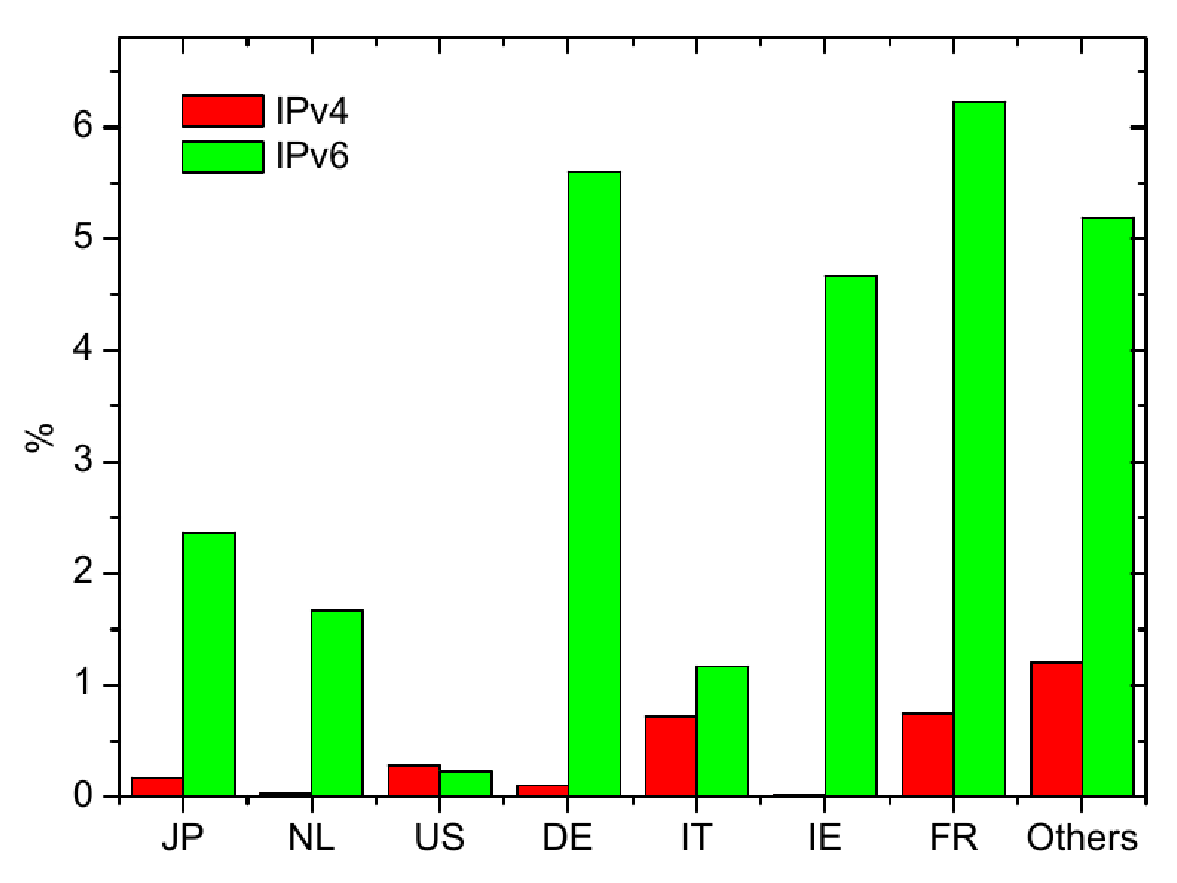
\includegraphics[width=2.5in]{packet_loss}
    \caption{IPv4 vs IPv4 packet loss rate for some representative countries
    when reached from China (2005).}
    \label{fig:packet_loss}
\end{figure}

\begin{figure}[!t]
    \centering
    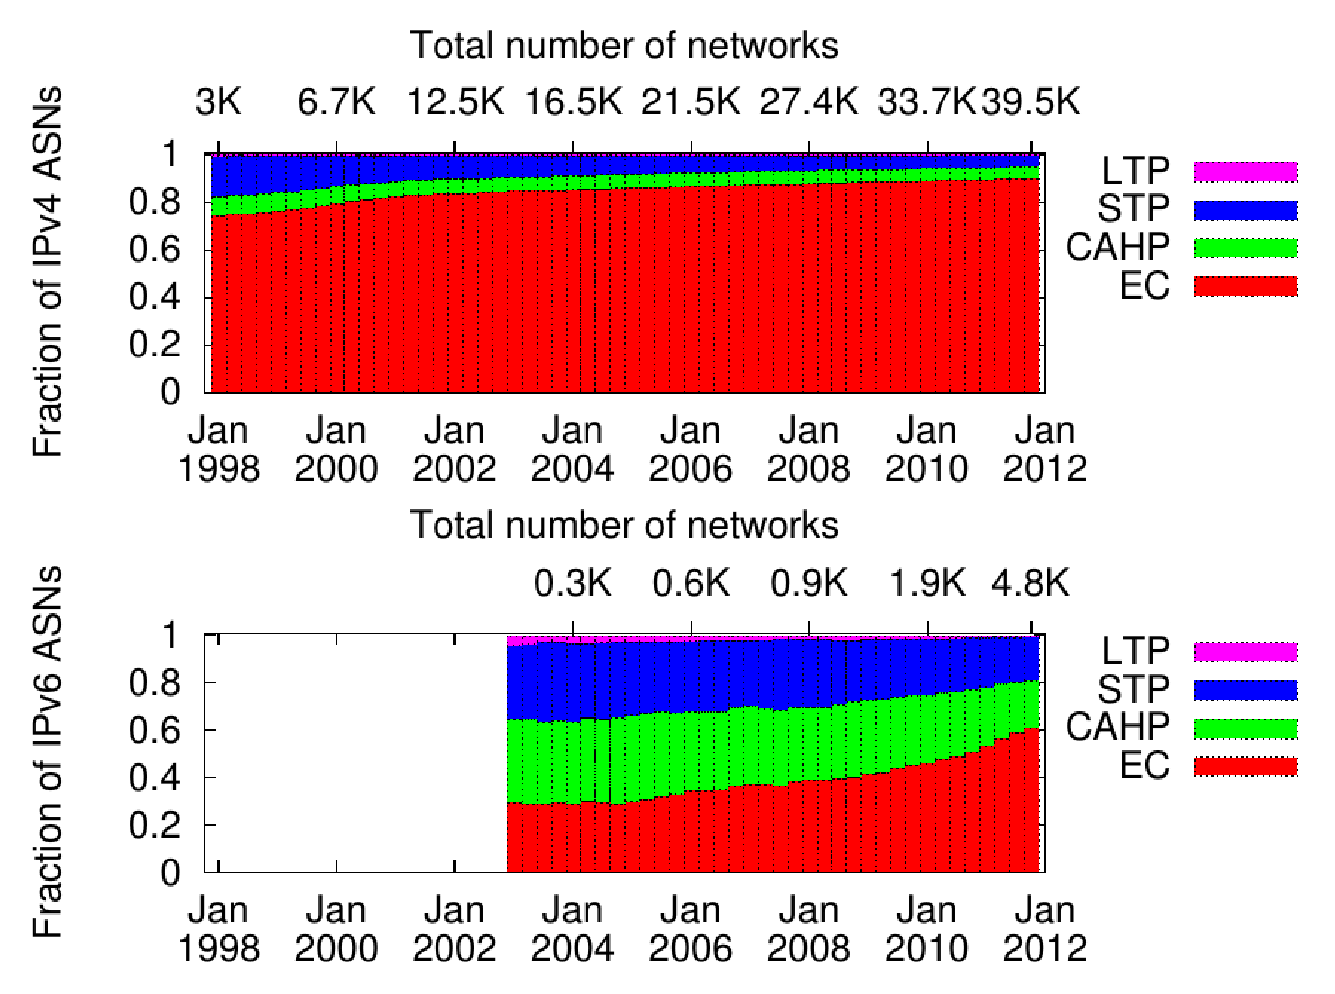
\includegraphics[width=2.5in]{as_types}
    \caption{Global ASes classification (see \ref{early} for classes
    definitions) over time for IPv4 and IPv6.}
    \label{fig:as_types}
\end{figure}

\section{IPv6 penetration}
\label{penetration}

\subsection{End-user penetration}
\label{client_penetration}

Google, Inc. engineers are measuring their users IPv6 adoption since
mid-2008. \\
They do so by adding for a random subset of their visitors a Javascript
\enquote{spyware} to their search engine.
This bunch of code executes a simple non-cached HTTP query to a dual-stack
(IPv6 + IPv4) server. By logging these queries, they are able to
estimate the number of clients which will be using IPv6 to access a dual-stacked
website\cite{paper2}. \\
While being executed on a large and scattered population, this measure doesn't
give any hint over clients' IPv6 support. If an user is accessing the dual-stack
website using IPv4, that doesn't imply that the user doesn't support IPv6. Some
operating systems and browsers prefer IPv4 over IPv6: Windows XP prefers IPv4
over IPv6 and newer versions of Windows prefer IPv4 to an available IPv6
tunnel. \\
By September 2009, they measured an IPv6 hit proportion of around 0.25\% with a
majority of users using 6to4 tunnels. This can be contrasted with the latest
measurements from the same team that exceed 3\% with about no tunnel
connection. Since mid-2010, IPv6 usage is clearly taking an exponential 
growth\cite{google:ipv6}. \\
Interestingly, as of 2008, the French ISP Free was the worldwide leading source
of IPv6 hits for Google (55\%). Free was also the first ISP to deploy IPv6 using
the 6rd tunneling mechanism\cite{free:6rd}. Other hits were mainly coming from
educational institutions.

\subsection{Network penetration}
\label{network_penetration}

By analyzing some historical BGP data lasting from 2003 to 2012, \cite{paper4}
noticed that the number of IPv6 ASes and AS links have followed a linear
growth until 2008 and have since started to increase by following an exponential
curve. This is interesting because the same measurements for IPv4 have followed
a linear growth during the same period. Using newer
numbers\cite{ripe:ipv6stats}, we can see that this growth have since
slowed down. The proportion of ASes announcing an IPv6 prefix had increased by
235\% between January 2010 and January 2012 while it has only increased by 135\%
between January 2012 and January 2014. Remember that as of today (March 2014),
17.5\% of global ASes are announcing an IPv6 prefix.\\

The major transit operator in IPv6 is \textit{Hurricane Electric} (HE), being a
relay on most BGP paths. This is to be contrasted with IPv4 for which
\textit{Level 3} is the major operator. As the presence of HE is predominant in
the still small IPv6 network, any changes in its peering policy inducts
noticeable events. Since HE opened their peering policy around
2007\cite{he:peering}, their growing importance in the IPv6 topology (by the
\enquote{eruption} of a large number of direct links to content providers)
produced a noticeable reduction of the measured average IPv6 BGP path length.
The average IPv6 BGP path length is since lightly smaller than the IPv4 one
(2.8 hops vs 3.2 hops, respectively).


\section{IPv6 performances}
\label{performances}

\subsection{Path is the major issue}
\label{path_issue}

To compare IPv6 to IPv4 performances, \cite{paper3} and \cite{paper4} probed the
top 1M Alexa websites that supported the two protocols from a set of different
locations. \\
To isolate potential differences and their cause, they grouped probed websites
in three categories depending on the nature of the
AS which are announcing them in both protocol :

\begin{enumerate}
    \item websites which share the same AS and BGP path in IPv4 and IPv6 ;
    \label{SP}
    \item websites which share the same AS in IPv4 and IPv6 but not the same
    BGP path ;
    \label{DP}
    \item websites which don't have the same AS in IPv4 and IPv6.
    \label{DL}
\end{enumerate}

As \ref{SP}) websites are sharing the same BGP path for IPv4 and IPv6, they
inferred that tunnels should not be responsible in any performance differences
between the two protocols. After excluding some outliners from this category
(websites which are significantly slower than other websites in the same AS for
a given protocol, explained by some infrastructure differences within the AS),
they were unable to find any noticeable speed variation between IPv4 and IPv6.
That supports the conclusion that IPv4 and IPv6 perform equally if the followed
path is identical. \\
By comparing \ref{DP}) and \ref{DL}) websites using a similar
procedure, they found deficiencies in IPv6 performances when the
number of hops was significantly lower or higher than in the corresponding IPv4
path. A lower number of hops can be explained with the presence of a tunnel
whereas a higher one implies either the absence of some links in the smaller
IPv6 graph or the inability of a CDN to provide content over IPv6
(mostly for \ref{DL}) websites which are not in the same location depending on
the used protocol, the IPv6 location being the \enquote{raw} website whereas the
IPv4 location is referencing the geographically closer CDN).\\

Knowing that the major IPv6 performance issues arise when the IPv6 AS path
differs from the IPv4 one, \cite{paper4} measured in 2012 the portion of
dual-stack servers which were reachable using a same AS path for IPv4 and IPv6.
At that time, more than 40\% of them were reached using the same path (10\%-20\%
were in 2004) while 60\% to 70\% of them were reached using an IPv4
path on which every crossed link is also present on the IPv6 graph (IPv6 routing
algorithms choose another path for some reasons)\footnote{
As a matter of precision, almost every IPv6 ASes and AS links is also on the
IPv4 graph. This observation about AS links leads to the conclusion that IPv6 on
IPv4 tunnels do not exist anymore at the core of the network.}.
These last observations confirm the assertion from \ref{early}
that the IPv6 adoption is now mostly lagging on the edges of the network, not at
its core.

\subsection{Routing dynamics}

By comparing the average BGP convergence delay and the average number of route
updates observed by ASes in the IPv4 and IPv6 topologies, \cite{paper4}
concluded that the work involved for routing updates by IPv6 topology changes is
becoming as similar to the work needed in the IPv4 topology as the IPv6 network
approaches the IPv4 size. \\
Since 2007 and after the removal of some outliners, the BGP convergence delay of
both networks is around 60-80 seconds while the average number of daily route
updates, when normalized by the number of ASes in the network, is roughly the
same. Routing dynamic overheads in the present-day IPv6 network are thus
equivalent to those found in the IPv4 network. The average number of updates was
an order of magnitude higher in the early stages of the IPv6 network, probably
because of the lack of isolation and of some immature routing policies.

\subsection{Perceived latency from the client side}

Using the method described in \ref{client_penetration}, Google engineers measured
the perceived latency from the browser point of view. \\
They measured the delta-time between the moment the search page with the
Javascript probe have been sent and the moment they received their hit on the
server . \\
That way, they were able to compare the latency between clients using IPv4 and
those using IPv6. \\
Results have been plotted on Fig. \ref{fig:google_latency} as a cumulative
distribution. \textit{IPv4-only} is for server-enforced IPv4 hits (the IPv6 of
the dual-stack server hasn't been provided), \textit{IPv4-dualstack} for
client-chosen IPv4 hits, \textit{IPv6-dualstack} for IPv6 hits and
\textit{IPv6-norelay} for IPv6 hits excluding those using tunnels (when
detected). \\
First, there is absolutely no difference between \textit{IPv4-only} and
\textit{IPv4-dualstack} which means that providing an IPv6 access to a website
doesn't increase its perceived latency for IPv4 users.
Secondly, we see that the IPv6 latency is slightly lower, especially
when not taking into account relayed clients. This surprising result isn't
probably caused by the IPv6 protocol itself but by IPv6 ISPs which have better
networks on average.

\begin{figure}[!t]
    \centering
    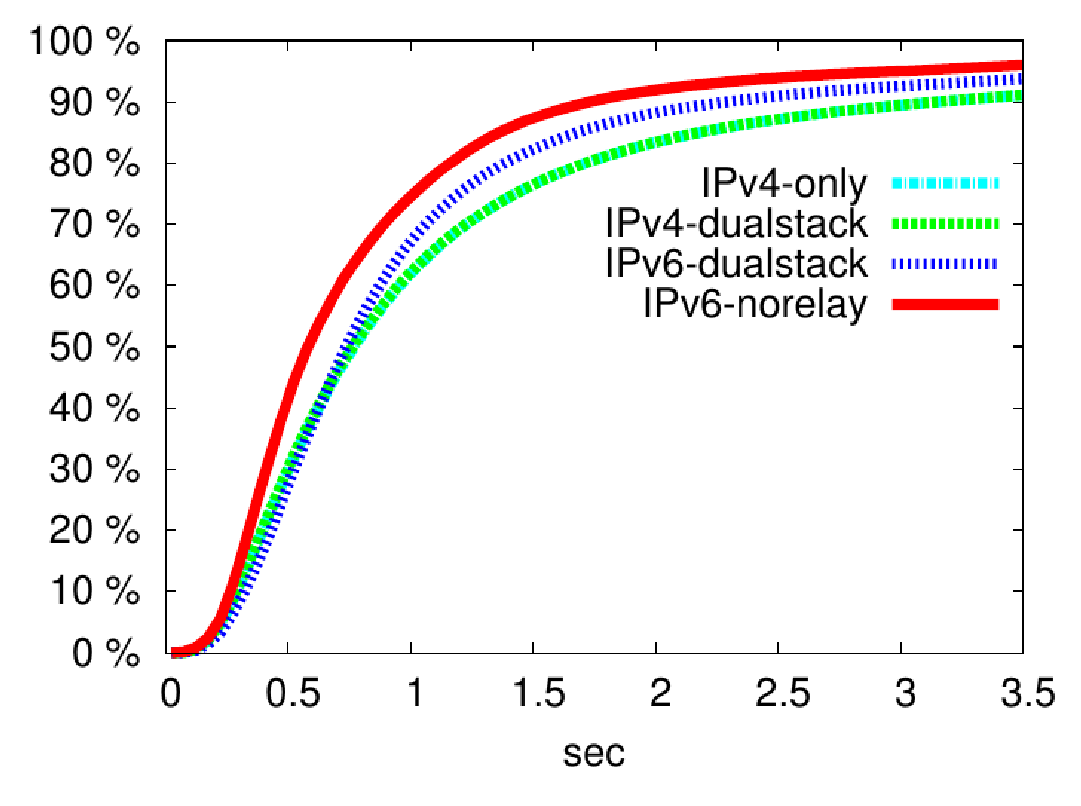
\includegraphics[width=2.5in]{google_latency}
    \caption{Cummulative distribution of hit latency on the Google service. The
    IPv4-only and IPv4-dualstack plots are roughly indistinguishable (2010).}
    \label{fig:google_latency}
\end{figure}

\section{Conclusion}

For the past five years, the IPv6 network has involved from an highly sparse
network, relying a lot of tunneling, into an increasingly mature network,
becoming more and more comparable to IPv4 in its topology, especially at its
core. \\
As described in \ref{path_issue}, \cite{paper3} and \cite{paper4} established 
that any observable performance deficiency of IPv6 hasn't any correlation with
the protocol in itself or with its implementations but with the maturity of the
network. \\
Studies also established that the IPv6 topology is catching increasingly faster
its IPv4 complement. However, as these studies start to aging, it will be
interesting to measure if the global IPv6 graph is still exponentially catching
up the complexity of its IPv4 counterpart, especially on the edges of the
network. \\
Once the IPv6 mesh of peering points will have become similar to the IPv4 one,
we will definitely be able to rank IPv4 as a residue of the past.

% An example of a floating figure using the graphicx package.
% Note that \label must occur AFTER (or within) \caption.
% For figures, \caption should occur after the \includegraphics.
% Note that IEEEtran v1.7 and later has special internal code that
% is designed to preserve the operation of \label within \caption
% even when the captionsoff option is in effect. However, because
% of issues like this, it may be the safest practice to put all your
% \label just after \caption rather than within \caption{}.
%
% Reminder: the "draftcls" or "draftclsnofoot", not "draft", class
% option should be used if it is desired that the figures are to be
% displayed while in draft mode.
%
% \begin{figure}[!t]
% \centering
% \includegraphics[width=2.5in]{myfigure}
% where an .eps filename suffix will be assumed under latex, 
% and a .pdf suffix will be assumed for pdflatex; or what has been declared
% via \DeclareGraphicsExtensions.
% \caption{Simulation Results.}
% \label{fig_sim}
% \end{figure}

% Note that IEEE typically puts floats only at the top, even when this
% results in a large percentage of a column being occupied by floats.

% An example of a double column floating figure using two subfigures.
% (The subfig.sty package must be loaded for this to work.)
% The subfigure \label commands are set within each subfloat command,
% and the \label for the overall figure must come after \caption.
% \hfil is used as a separator to get equal spacing.
% Watch out that the combined width of all the subfigures on a 
% line do not exceed the text width or a line break will occur.
%
%\begin{figure*}[!t]
%\centering
%\subfloat[Case I]{\includegraphics[width=2.5in]{box}%
%\label{fig_first_case}}
%\hfil
%\subfloat[Case II]{\includegraphics[width=2.5in]{box}%
%\label{fig_second_case}}
%\caption{Simulation results.}
%\label{fig_sim}
%\end{figure*}
%
% Note that often IEEE papers with subfigures do not employ subfigure
% captions (using the optional argument to \subfloat[]), but instead will
% reference/describe all of them (a), (b), etc., within the main caption.


% An example of a floating table. Note that, for IEEE style tables, the 
% \caption command should come BEFORE the table. Table text will default to
% \footnotesize as IEEE normally uses this smaller font for tables.
% The \label must come after \caption as always.
%
%\begin{table}[!t]
%% increase table row spacing, adjust to taste
%\renewcommand{\arraystretch}{1.3}
% if using array.sty, it might be a good idea to tweak the value of
% \extrarowheight as needed to properly center the text within the cells
%\caption{An Example of a Table}
%\label{table_example}
%\centering
%% Some packages, such as MDW tools, offer better commands for making tables
%% than the plain LaTeX2e tabular which is used here.
%\begin{tabular}{|c||c|}
%\hline
%One & Two\\
%\hline
%Three & Four\\
%\hline
%\end{tabular}
%\end{table}


% Note that IEEE does not put floats in the very first column - or typically
% anywhere on the first page for that matter. Also, in-text middle ("here")
% positioning is not used. Most IEEE journals use top floats exclusively.
% Note that, LaTeX2e, unlike IEEE journals, places footnotes above bottom
% floats. This can be corrected via the \fnbelowfloat command of the
% stfloats package.







% if have a single appendix:
%\appendix[Proof of the Zonklar Equations]
% or
%\appendix  % for no appendix heading
% do not use \section anymore after \appendix, only \section*
% is possibly needed

% use appendices with more than one appendix
% then use \section to start each appendix
% you must declare a \section before using any
% \subsection or using \label (\appendices by itself
% starts a section numbered zero.)
%


\appendices

% can use a bibliography generated by BibTeX as a .bbl file
% BibTeX documentation can be easily obtained at:
% http://www.ctan.org/tex-archive/biblio/bibtex/contrib/doc/
% The IEEEtran BibTeX style support page is at:
% http://www.michaelshell.org/tex/ieeetran/bibtex/
%\bibliographystyle{IEEEtran}
% argument is your BibTeX string definitions and bibliography database(s)
%\bibliography{IEEEabrv,../bib/paper}
%
% <OR> manually copy in the resultant .bbl file
% set second argument of \begin to the number of references
% (used to reserve space for the reference number labels box)

\bibliographystyle{IEEEtran}
\bibliography{report}

\end{document}


